\documentclass{article}
\usepackage{graphicx} % Required for inserting images
\usepackage{amsmath}
\usepackage[margin=1in]{geometry}
\usepackage{parskip}
\usepackage{tikz}
\usetikzlibrary{arrows.meta,calc,backgrounds,decorations.pathreplacing}

\title{$\epsilon$-Cohesive Cores in Bipartite Graphs}
\author{Kiyaan Pillai}
\date{October 2026}

\begin{document}

\maketitle

\section{Introduction}

Choose $\theta$, $\epsilon$, and a distance function $d$. Let $G = (L, R, E)$. Choose a set of left-hand vertices $\mathcal{L} \subseteq L$. Let $N(\ell) \subseteq R$ be the neighbors of a single node. Let $N(\mathcal{L}) \subseteq R$ be the union of the neighbors of vertices in $\mathcal{L}$, where a vertex $r$ is a neighbor of some $\ell \in \mathcal{L}$ if there exists an edge between $\ell$ and $r$. The diameter $M$ of a subgraph $\mathcal{L} \in L$ is the smallest number such that every $\ell \in \mathcal{L}$ can select a subset $A_\ell \subseteq N(\ell)$ with
$|A_\ell| \ge \theta$, with the maximum pairwise distance of the union of these subsets.

$$M_\mathcal{L} = \min_{(A_\ell)_{\ell\in\mathcal{L}}} \; \max_{r_1,r_2 \in \bigcup_\ell A_\ell} d(r_1,r_2)$$

where each $A_\ell \subseteq N(\ell)$ and $|A_\ell|\ge\theta$. $\mathcal{L}$ is an $\epsilon$-cohesive core if $M_\mathcal{L} < \epsilon$.

If $|N(\mathcal{L})| = 1$, then $M_\mathcal{L} = 0$.

If for a given $\mathcal{L} \subseteq L$, $M < \epsilon$ and every vertex has at least $\theta$ neighbors, then $\mathcal{L}$ is an $\epsilon$-cohesive core. Find the largest $\epsilon$-cohesive core.

One use case is for recommendation systems. Bicliques have been used to detect similar users and suggest products that those users bought [1]. However, the biclique is unnecessarily restrictive, and $\gamma$-quasi-bicliques [2] as well as $k$-edge defective bicliques [3] have been proposed to recover slightly noisy structure. However, both models reject structure where users interact with slightly similar, though not identical, products, even though this structure could be useful.

\begin{figure}[h]
\centering
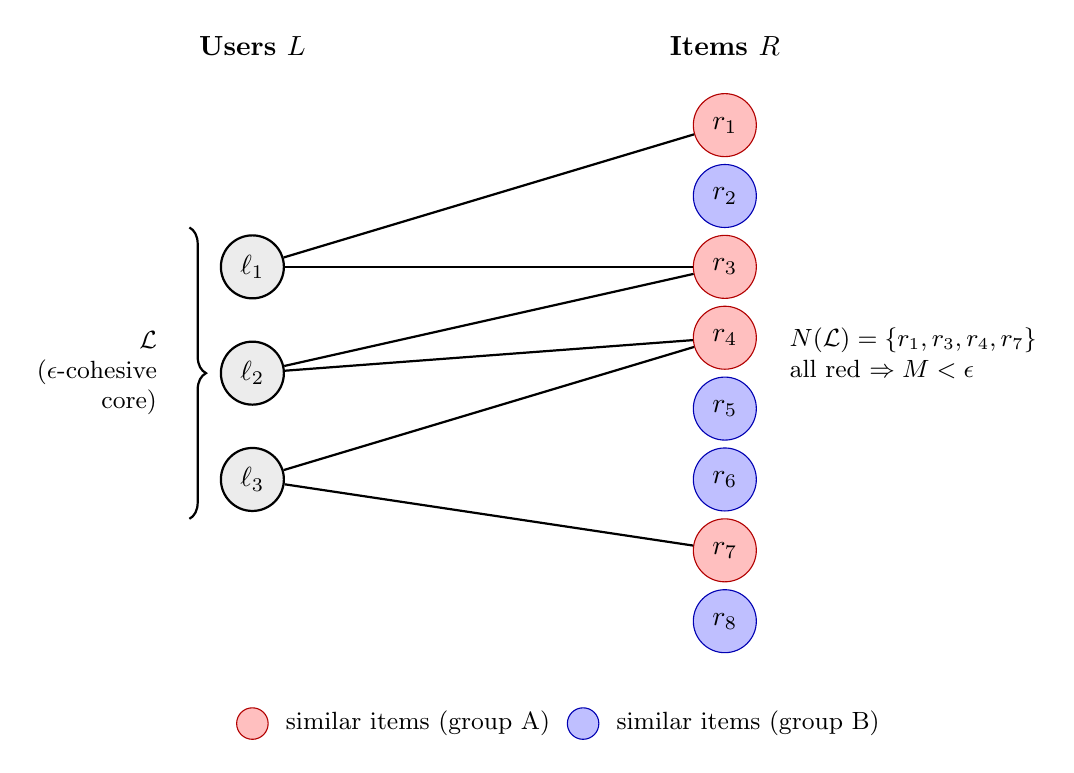
\begin{tikzpicture}[
    >=Stealth,
    user/.style={circle, draw=black, thick, fill=gray!15, minimum size=8mm, inner sep=0pt},
    red item/.style={circle, draw=red!70!black, fill=red!25, minimum size=8mm, inner sep=0pt},
    blue item/.style={circle, draw=blue!70!black, fill=blue!25, minimum size=8mm, inner sep=0pt},
    coreedge/.style={black, thick}
]
 
% ---- Column headings (absolute positions) ----
\node[font=\bfseries] at (0,7.3)  {Users $L$};
\node[font=\bfseries] at (6,7.3)  {Items $R$};
 
% ---- Left vertices: the core $\mathcal{L}$ ----
\node[user] (u1) at (0,4.5)  {$\ell_1$};
\node[user] (u2) at (0,3.15) {$\ell_2$};
\node[user] (u3) at (0,1.8)  {$\ell_3$};
 
% ---- Right vertices: colour = similarity group; red and blue are interleaved ----
\node[red item]  (v1) at (6,6.3) {$r_1$};
\node[blue item] (v2) at (6,5.4) {$r_2$};
\node[red item]  (v3) at (6,4.5) {$r_3$};
\node[red item]  (v4) at (6,3.6) {$r_4$};
\node[blue item] (v5) at (6,2.7) {$r_5$};
\node[blue item] (v6) at (6,1.8) {$r_6$};
\node[red item]  (v7) at (6,0.9) {$r_7$};
\node[blue item] (v8) at (6,0.0) {$r_8$};
 
% ---- Edges ($\theta=2$): each user has 2 neighbours, all red ----
\draw[coreedge] (u1)--(v1);
\draw[coreedge] (u1)--(v3);
\draw[coreedge] (u2)--(v3);
\draw[coreedge] (u2)--(v4);
\draw[coreedge] (u3)--(v4);
\draw[coreedge] (u3)--(v7);
 
% ---- Brace and label for $\mathcal{L}$ ----
\draw[decorate, decoration={brace, amplitude=6pt}, thick]
     (-0.8,5.0) -- (-0.8,1.3) node[midway, left=8pt, align=right, font=\small]
     {$\mathcal{L}$\\($\epsilon$-cohesive\\core)};
 
% ---- Annotation for $N(\mathcal{L})$ ----
\node[font=\small, anchor=west, align=left] at (6.7,3.4)
     {$N(\mathcal{L})=\{r_1,r_3,r_4,r_7\}$\\ all red $\Rightarrow M<\epsilon$};
 
% ---- Legend ----
\node[red item, minimum size=4mm]  at (0,-1.3) {};
\node[anchor=west, font=\small] at (0.3,-1.3) {similar items (group A)};
\node[blue item, minimum size=4mm] at (4.2,-1.3) {};
\node[anchor=west, font=\small] at (4.5,-1.3) {similar items (group B)};
 
\end{tikzpicture}
\caption{Example with $\theta=2$. Same-colored items are within $\epsilon$ of each other, differently-colored items are not. Every user in $\mathcal{L}=\{\ell_1,\ell_2,\ell_3\}$ has at least $\theta$ neighbors and $N(\mathcal{L})$ contains only red items, so $M<\epsilon$. The users do not share a common neighborhood (no biclique larger than $2\times1$), and $6$ of the $12$ possible edges between $\mathcal{L}$ and $N(\mathcal{L})$ are missing, so a $\gamma$-quasi-biclique or $k$-edge defective biclique with small $\gamma$ or $k$ rejects $\mathcal{L}$. Our model recovers it because the items each user chose are similar, though not identical.}
\end{figure}

\section{Proof of NP-hardness}

I was not able to fully prove that this graph formulation is NP-hard. However, here is my intuition for a reduction:

Let $G = (V, E_G)$. Construct a bipartite graph $B = (L, R, E_B)$ where $L = V$, $R = V$, and edges exist between every $(\ell, r) \mathrel{\text{s.t.}} \ell = r$. In other words, the bipartite graph is entirely a matching. This reduction takes $\mathcal{O}(|V|)$ because it must create $2|V|$ vertices and $|V|$ edges, so it is therefore a polynomial-time reduction.

Fix $\epsilon = 2$, $\theta = 1$, and

\begin{equation}
d(r_1, r_2) = 
\begin{cases}
    0 & \text{if } r_1 = r_2 \\
    1 & \text{if } (r_1, r_2) \in E_G \mathrel{\text{or}} r_1 = r_2 \\
    3 & \text{otherwise}
\end{cases}
\end{equation}

Each vertex $\ell \in L$ has exactly one neighbor (itself), so with $\theta = 1$, every subset of $L$ satisfies the minimum degree constraint.

Because $d \in \{1, 3\}$ and $\epsilon = 2$, two vertices meet the similarity constraint iff they have an edge between them. Therefore, if $M < \epsilon$, then all vertices in $N(\mathcal{L})$ must have an edge between every other vertex, and therefore they must form a clique. Finding the maximum number of vertices $\ell \in \mathcal{L}$ is equivalent to finding the maximum number of clique vertices $r \in V$, because the bipartite graph has a one-to-one matching. Therefore, for a given $\ell \in \mathcal{L}$, $N(\ell) = \{\ell\}$.

Because two vertices are considered similar iff they have an edge between them, finding a group of vertices that are all similar to each other is equivalent to finding a clique. Therefore, finding the maximum $\epsilon$-cohesive core is equivalent to finding the maximum clique in $G$.

I believe this reduction from Max CLIQUE establishes NP-hardness of the optimization variant of this problem. I would appreciate feedback on whether this seems intuitively valid as I try to formalize this proof.

\section{Literature Review}

To my knowledge, this exact formulation has not been studied.

It is most similar to Yao et al. [1]. They proposed a biclique in which vertices on the same side are similar. They define two vertices as being similar if the Jaccard similarity of their neighbors is $\geq$ some threshold $\epsilon$. However, Yao et al. do not generalize this similarity to some arbitrary distance function, and they require the model to be a biclique.

The formulation may also be thought of as a mapping of the geo-social group (GSG) proposed by Li \& Zlatanova [4]. This problem relates to a graph where each node has an associated 2D coordinate pair. The GSG is the largest group of nodes whose coordinates all fall within an enclosing circle of radius $\leq \gamma$ for some threshold $\gamma$.

\section{Future Idea}

Set an overlap parameter $I$ such that $|\bigcap_{\ell \in \mathcal{L}}N(\ell)| \geq I$. For example, if $I = 1$, everyone has to have bought at least 1 exactly identical product.

\section{References}

[1]
K. Yao, L. Chang, and J. X. Yu, “Identifying Similar-Bicliques in Bipartite Graphs,” Proceedings of the VLDB Endowment, vol. 15, no. 11, pp. 3085–3097, Jul. 2022, doi: 10.14778/3551793.3551854.

[2]
K. Sim, J. Li, V. Gopalkrishnan, and G. Liu, “Mining Maximal Quasi‐Bicliques: Novel Algorithm and Applications in the Stock Market and Protein Networks,” Statistical Analysis and Data Mining: The ASA Data Science Journal, vol. 2, no. 4, pp. 255–273, Oct. 2009, doi: 10.1002/sam.10051.

[3]
D. Cui, R. Li, Q. Dai, H. Qin, and G. Wang, “On the Efficient Discovery of Maximum $K$-Defective Biclique,” arXiv.org. Accessed: Sep. 24, 2026. [Online]. Available: https://arxiv.org/abs/2506.16121

[4]
W. Li and S. Zlatanova, “Significant Geo-Social Group Discovery Over Location-Based Social Network,” Sensors (Basel), vol. 21, no. 13, p. 4551, Jul. 2021, doi: 10.3390/s21134551.

\end{document}